\documentclass{article}

% Language setting
% Replace `english' with e.g. `spanish' to change the document language
\usepackage[english]{babel}

% Set page size and margins
% Replace `letterpaper' with `a4paper' for UK/EU standard size
\usepackage[letterpaper,top=2cm,bottom=2cm,left=3cm,right=3cm,marginparwidth=1.75cm]{geometry}

% Useful packages
\usepackage{amsmath}
\usepackage{amssymb}
\usepackage{graphicx}
\usepackage{inconsolata}
\usepackage{minted}
\usepackage[colorlinks=true, allcolors=blue]{hyperref}

\title{Innleveing 1}

\begin{document}
\maketitle

\section{Oppgave 1}

a) A og B

b) Usikker men gjetter C 

c) A

d) m/s

e) B

f) A

g) B

\section{Oppgave 2}

a) B

b) B

c) C

d) D

e) C

f) D

\section{Oppgave 3}

a) B

b) Gjetter B

c) Gjetter A

d) D

e) D

f) Usikker

g) Gjetter A

\section{Oppgave 3}

a) B

b) Gjetter B

c) Gjetter A

d) D

e) D

f) Usikker

g) Gjetter A

\section{Oppgave 4}

\subsection{a)}

Jeg løser denne oppgaven ved å integrere farsfunksjonen til ballen for å finne posisjon for tid

$$\int v(t) = \int 8.5 m/s - 9.81 m/s^2 \cdot t - \frac{1}{2} \cdot 9.81 m/s^2 \cdot t^2 = p(t)$$

Videre kan jeg løse $v(t)=0$ og sette det i $p(t)$

$v(t) = 0 \rightarrow t = \frac{840}{981}s$

$p(t)=3.68 m$

Det høyeste punktet til ballen er $3.68m$

\subsection{b)} 

Jeg bruker det jeg fikk fra forrige oppgaven

$$v(t) = 0 \rightarrow t = \frac{840}{981}s \approx 0.87s$$

Ballen bruker $0.87s$ for å komme til det øverste punktet i banen setting

\subsection{c)}

For å finne ut av hvor lang tid ballen bruker før den er tilbake ved Maries hånd kan vi løse likningen $p(t)=0m$

\begin{align*}
    p(t) = 0 \\
    t = 0 \lor t = \frac{1700}{981} \text{forkaster $t=0$ løsningen} \\
    t = \frac{1700}{981} \approx 1.73
\end{align*}

\subsection{d)}

Vi vet når ballen trefer hånden som er etter 1,73 sekunder. 
Da kan vi finne farten ved å sette dette i fartsformelen

$v(1.73) = -8.5 m/s$

Farten er $8.5$ m7s nedover når ballen treffer hånden til Marie

\subsection{e)}

Vi har formelen for posisjon så vi kan sette in 2,12 sekunder i den for å finne hvor høyt Marie kastet ballen fra

$f(2.12) \approx -4.03 m$

Marie kaster ballen fra $4.03$ meter over bakken

\subsection{f)}

\begin{figure}[H]
    \centering
    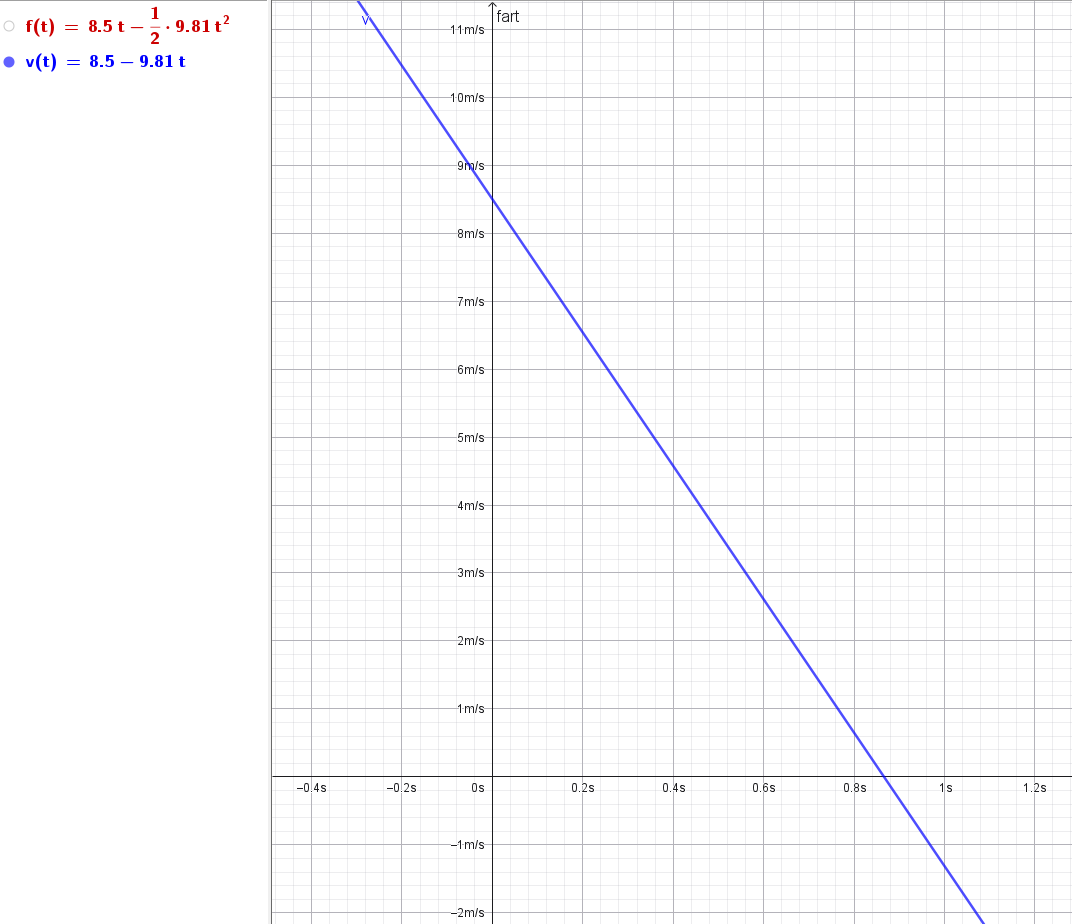
\includegraphics[width=0.7\textwidth]{bilder/2f.png}
    \caption{Fartsgrafen}
\end{figure}

\subsection{g)}

\begin{figure}[H]
    \centering
    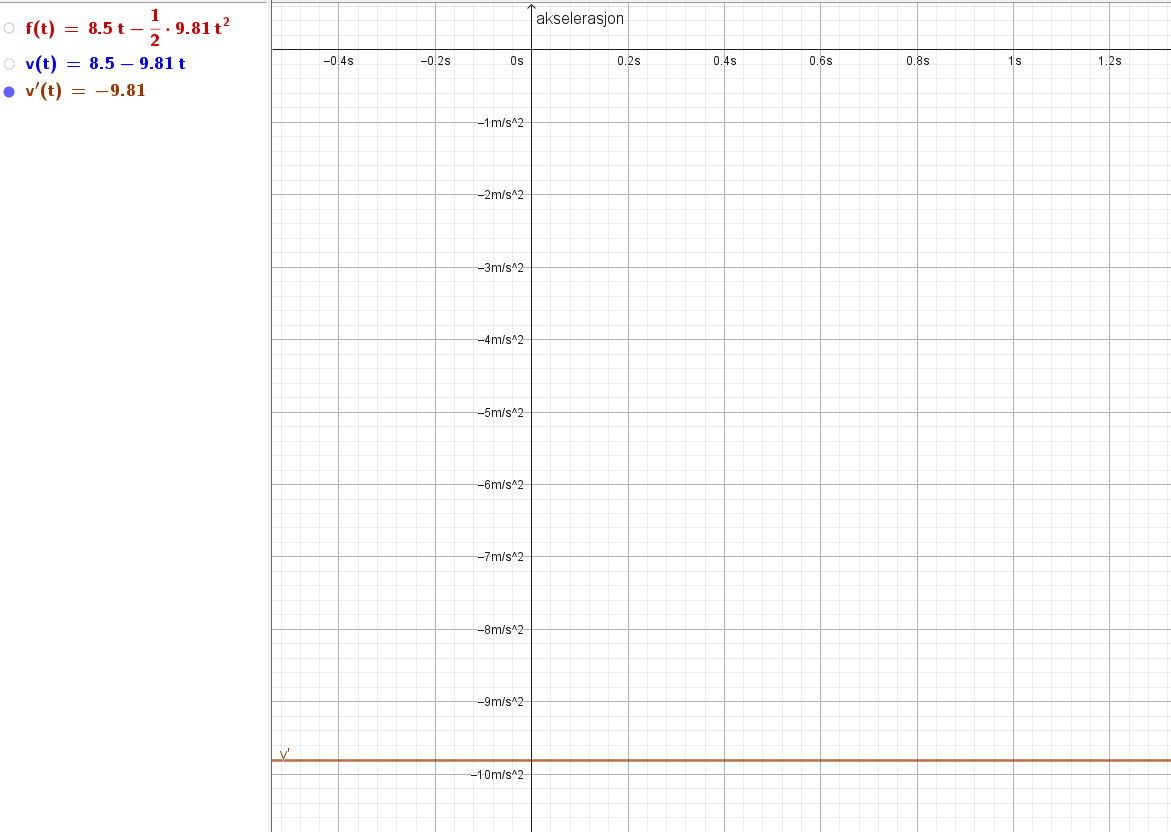
\includegraphics[width=0.7\textwidth]{bilder/2g.png}
    \caption{Akselerasjonsgrafen}
\end{figure}

\section{Oppgave 5}

h)

Vi kan finne den potensielle energien ved: $mgh$

$$0.15 kg * 5m * 9.81 m/s^2 = 7.35 J$$

Den potensielle energien til ballen når den når toppunktet er 7,35 Joule

i)

Den kinetiske energien er den samme som den potensielle energien i toppunktet.

$E_p = E_k = 7.35 J$

Den kinetiske energien er 7,35 Joule når den forlater hånden hennes

j)

Får å finne farten kan vi løse likningen: $E_p = E_k$

\begin{align*}
    E_p &= E_k \\
    mgh &= \frac{1}{2} v^2 * m \\
    0.15 kg * 5m * 9.81 m/s^2 = \frac{1}{2} * v^2 m^2/s^2 * 0.15 kg \\
    \frac{0.15 kg * 5m * 9.81 m/s^2}{\frac{1}{2} * 0.15 kg} &= v^2 m^2 / s^2 \\
    \text{så kan kan jeg kvadrere for å finne farten} \\
    \sqrt{\frac{0.15 kg * 5m * 9.81 m/s^2}{\frac{1}{2} * 0.15 kg}} &= v \\
    v \approx 9.90 m/s
\end{align*}

Farten til ballen når den forlater hånden hennes er $9.90 m/s$

k)

Marie utfører at arbeid på $7.35J$ på ballen

l) 

Vi kan finne kraften hun bruker ved å dele energien på distansen hun bruker å akselerere ballen

$\frac{0.150 kg * 9.81 m/s^2 * 5.00 m}{0.200 m} \approx 36.768N$

Hun bruker $36.768N$ på ballen

m)

\begin{figure}[H]
    \centering
    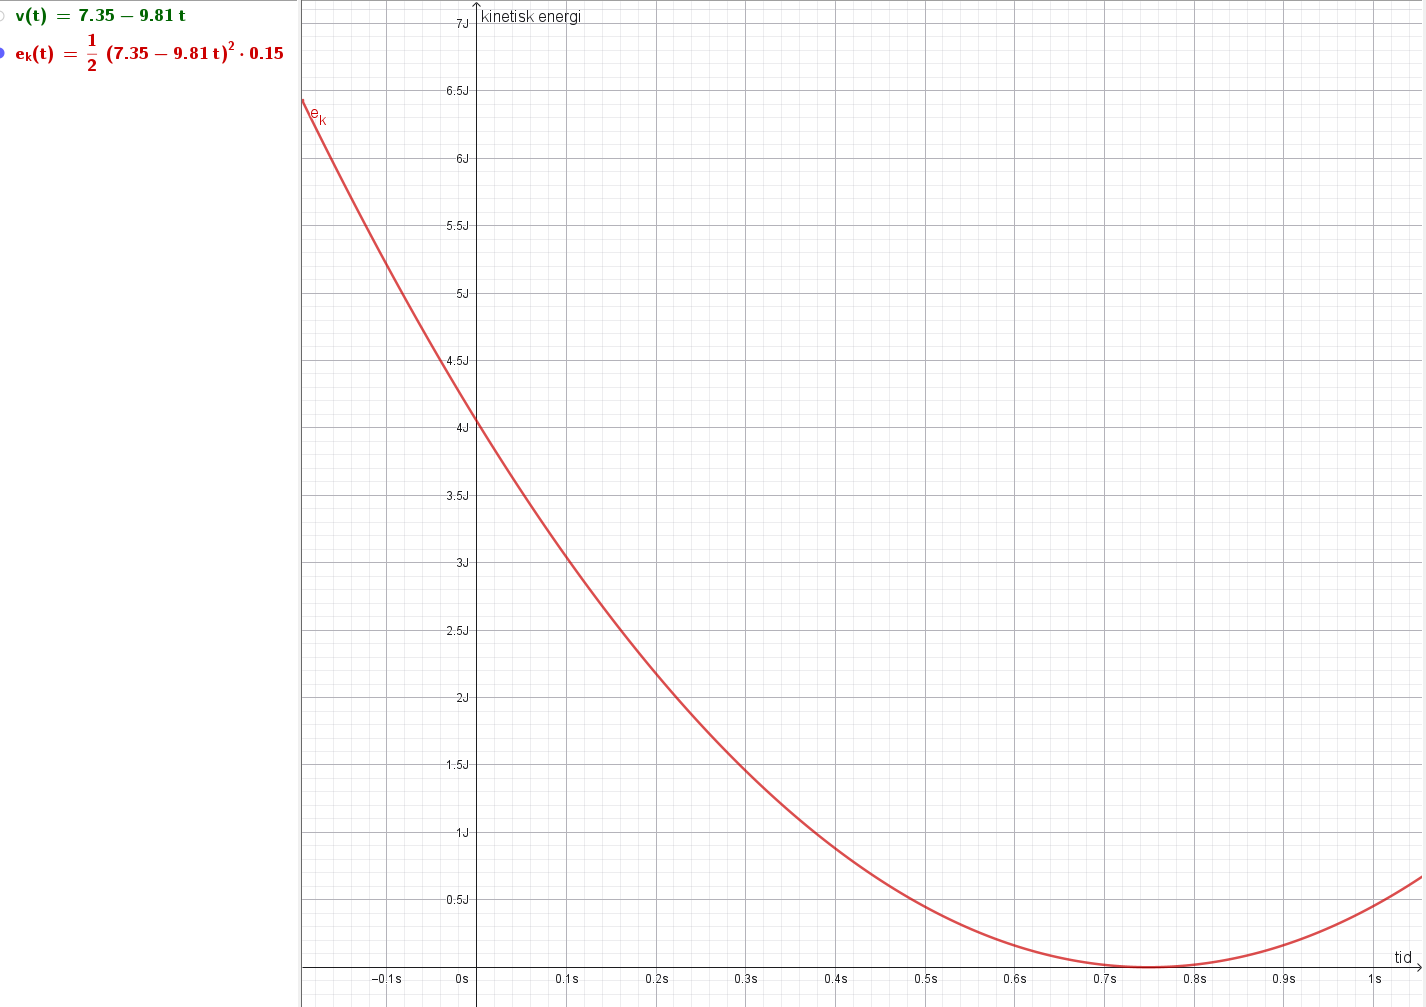
\includegraphics[width=0.7\textwidth]{bilder/4m.png}
    \caption{Graf over kinetisk energi}
\end{figure}

n)

\begin{figure}[H]
    \centering
    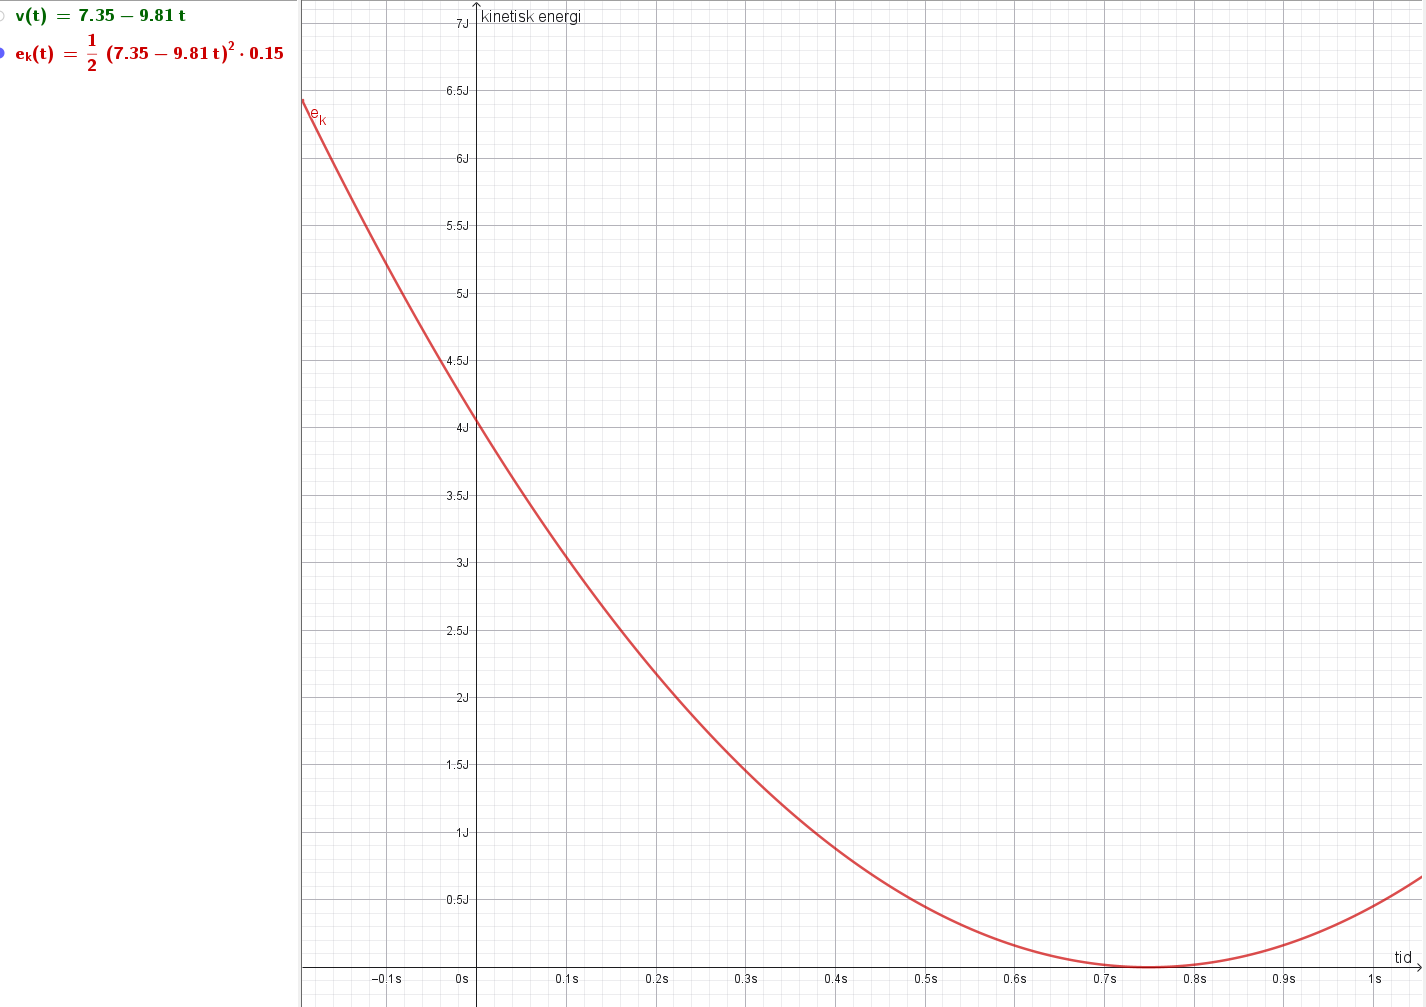
\includegraphics[width=0.7\textwidth]{bilder/4m.png}
    \caption{Energigraf}
\end{figure}

o)

Jeg tar utganspunkt i den potensielle energien

\begin{align*}
    0.150 kg * 9.81m/s * 5m - 0.150 kg 9.81 m/s 4m = 1.471J
\end{align*}

Luftmotsanden har gjort er arbeid på $1.471J$ på ballen
 
\bibliographystyle{alpha}
\bibliography{sample}

\end{document}
